\section{The ladder: further details}
\label{app:ladder-more}

This section supplements Section~\ref{sec:ladder} of the paper.
Table~\ref{tab:ladder-splits} lists the three splits of every length.
Table~\ref{tab:ladder-lengths} gives, for every length and seed, the final
accuracy of the arm that builds answers everywhere and of the self-paced
arm, with the novelty the self-paced arm measured and what it then did.

% Generated by `uv run python -m gainpred.ladder_paper`; do not edit by hand.
\begin{table}[htbp]
\centering
\caption{The three splits of every length 8--39, each written as left piece +
  right piece (digits).}
\label{tab:ladder-splits}
\small
\setlength{\tabcolsep}{3pt}
\begin{tabular}{rlll@{\hspace{1.5em}}rlll}
\toprule
\multicolumn{4}{c}{8--23 digits} & \multicolumn{4}{c}{24--39 digits} \\
\cmidrule(lr){1-4}\cmidrule(lr){5-8}
Digits & Split 1 & Split 2 & Split 3 & Digits & Split 1 & Split 2 & Split 3 \\
\midrule
8 & 3 + 5 & 4 + 4 & 5 + 3 & 24 & 11 + 13 & 12 + 12 & 13 + 11 \\
9 & 3 + 6 & 4 + 5 & 5 + 4 & 25 & 11 + 14 & 12 + 13 & 13 + 12 \\
10 & 4 + 6 & 5 + 5 & 6 + 4 & 26 & 12 + 14 & 13 + 13 & 14 + 12 \\
11 & 4 + 7 & 5 + 6 & 6 + 5 & 27 & 12 + 15 & 13 + 14 & 14 + 13 \\
12 & 5 + 7 & 6 + 6 & 7 + 5 & 28 & 13 + 15 & 14 + 14 & 15 + 13 \\
13 & 5 + 8 & 6 + 7 & 7 + 6 & 29 & 13 + 16 & 14 + 15 & 15 + 14 \\
14 & 6 + 8 & 7 + 7 & 8 + 6 & 30 & 14 + 16 & 15 + 15 & 16 + 14 \\
15 & 6 + 9 & 7 + 8 & 8 + 7 & 31 & 14 + 17 & 15 + 16 & 16 + 15 \\
\midrule
16 & 7 + 9 & 8 + 8 & 9 + 7 & 32 & 15 + 17 & 16 + 16 & 17 + 15 \\
17 & 7 + 10 & 8 + 9 & 9 + 8 & 33 & 15 + 18 & 16 + 17 & 17 + 16 \\
18 & 8 + 10 & 9 + 9 & 10 + 8 & 34 & 16 + 18 & 17 + 17 & 18 + 16 \\
19 & 8 + 11 & 9 + 10 & 10 + 9 & 35 & 16 + 19 & 17 + 18 & 18 + 17 \\
20 & 9 + 11 & 10 + 10 & 11 + 9 & 36 & 17 + 19 & 18 + 18 & 19 + 17 \\
21 & 9 + 12 & 10 + 11 & 11 + 10 & 37 & 17 + 20 & 18 + 19 & 19 + 18 \\
22 & 10 + 12 & 11 + 11 & 12 + 10 & 38 & 18 + 20 & 19 + 19 & 20 + 18 \\
23 & 10 + 13 & 11 + 12 & 12 + 11 & 39 & 18 + 21 & 19 + 20 & 20 + 19 \\
\bottomrule
\end{tabular}
\end{table}

% Generated by `uv run python -m gainpred.ladder_paper`; do not edit by hand.
\begin{table}[htbp]
\centering
\caption{For each length and seed: final accuracy (\%) of the third arm (Agreed)
  and of the self-paced arm (Paced) after their last round, the self-paced arm's
  novelty in its check before the length's round (\% of pair-agreed answers that
  differ from the direct answer), and whether it built or skipped the length.}
\label{tab:ladder-lengths}
\scriptsize
\setlength{\tabcolsep}{3pt}
\begin{tabular}{rrrrlrrrlrrrl}
\toprule
 & \multicolumn{4}{c}{Seed 5} & \multicolumn{4}{c}{Seed 6}
 & \multicolumn{4}{c}{Seed 7} \\
\cmidrule(lr){2-5}\cmidrule(lr){6-9}\cmidrule(lr){10-13}
Digits & Agreed & Paced & Novelty & Paced did & Agreed & Paced & Novelty
  & Paced did & Agreed & Paced & Novelty & Paced did \\
\midrule
8 & 98.8 & 99.7 & 96.5 & built & 100.0 & 100.0 & 82.5 & built & 100.0 & 100.0
  & 100.0 & built \\
9 & 99.0 & 99.6 & 100.0 & built & 100.0 & 100.0 & 100.0 & built & 99.9 & 100.0
  & 100.0 & built \\
10 & 98.8 & 99.4 & 85.8 & built & 100.0 & 100.0 & 72.5 & built & 100.0 & 100.0
  & 100.0 & built \\
11 & 98.8 & 99.6 & 100.0 & built & 100.0 & 99.9 & 100.0 & built & 100.0 & 100.0
  & 100.0 & built \\
12 & 99.0 & 99.6 & 92.8 & built & 100.0 & 100.0 & 0.57 & skipped & 100.0 & 100.0
  & 40.6 & built \\
13 & 98.6 & 99.2 & 100.0 & built & 100.0 & 100.0 & 99.0 & built & 100.0 & 100.0
  & 100.0 & built \\
14 & 98.2 & 99.3 & 15.3 & built & 100.0 & 99.9 & 1.3 & skipped & 100.0 & 100.0
  & 0.15 & skipped \\
15 & 98.3 & 99.3 & 97.7 & built & 100.0 & 100.0 & 92.8 & built & 100.0 & 100.0
  & 100.0 & built \\
\midrule
16 & 97.8 & 99.2 & 12.4 & built & 100.0 & 100.0 & 0.00 & skipped & 100.0 & 100.0
  & 23.5 & built \\
17 & 98.1 & 99.4 & 89.1 & built & 100.0 & 100.0 & 28.5 & built & 100.0 & 100.0
  & 100.0 & built \\
18 & 97.6 & 98.6 & 2.9 & built & 100.0 & 100.0 & 0.15 & skipped & 100.0 & 100.0
  & 0.00 & skipped \\
19 & 97.1 & 98.4 & 99.4 & built & 100.0 & 100.0 & 0.15 & skipped & 100.0 & 100.0
  & 12.2 & built \\
20 & 98.2 & 99.5 & 0.29 & skipped & 100.0 & 100.0 & 51.8 & built & 100.0 & 100.0
  & 0.00 & skipped \\
21 & 97.6 & 99.0 & 4.9 & built & 100.0 & 100.0 & 100.0 & built & 99.9 & 100.0
  & 69.5 & built \\
22 & 97.4 & 98.5 & 0.30 & skipped & 100.0 & 99.9 & 0.00 & skipped & 99.9 & 100.0
  & 0.00 & skipped \\
23 & 97.8 & 98.8 & 12.7 & built & 100.0 & 100.0 & 1.4 & skipped & 100.0 & 100.0
  & 73.6 & built \\
\midrule
24 & 97.5 & 99.0 & 0.00 & skipped & 100.0 & 100.0 & 71.1 & built & 100.0 & 100.0
  & 0.15 & skipped \\
25 & 96.7 & 98.4 & 0.75 & skipped & 100.0 & 100.0 & 100.0 & built & 99.9 & 100.0
  & 79.3 & built \\
26 & 97.0 & 98.6 & 77.8 & built & 99.9 & 100.0 & 0.00 & skipped & 99.9 & 100.0
  & 0.14 & skipped \\
27 & 96.2 & 98.0 & 100.0 & built & 100.0 & 100.0 & 0.14 & skipped & 100.0
  & 100.0 & 24.4 & built \\
28 & 96.2 & 98.4 & 0.60 & skipped & 99.9 & 99.9 & 9.6 & built & 100.0 & 99.8
  & 0.00 & skipped \\
29 & 96.4 & 97.9 & 12.1 & built & 100.0 & 100.0 & 94.3 & built & 100.0 & 100.0
  & 32.7 & built \\
30 & 96.6 & 98.0 & 0.44 & skipped & 100.0 & 100.0 & 0.14 & skipped & 99.8
  & 100.0 & 0.00 & skipped \\
31 & 96.0 & 98.0 & 2.5 & built & 100.0 & 100.0 & 0.43 & skipped & 100.0 & 100.0
  & 1.3 & skipped \\
\midrule
32 & 95.0 & 97.9 & 0.30 & skipped & 100.0 & 100.0 & 2.3 & built & 99.9 & 100.0
  & 42.2 & built \\
33 & 95.7 & 97.8 & 1.3 & skipped & 100.0 & 100.0 & 66.1 & built & 99.9 & 100.0
  & 99.4 & built \\
34 & 96.0 & 98.0 & 1.2 & skipped & 100.0 & 100.0 & 0.59 & skipped & 100.0
  & 100.0 & 0.00 & skipped \\
35 & 95.2 & 97.6 & 75.1 & built & 99.9 & 100.0 & 7.1 & built & 100.0 & 100.0
  & 0.71 & skipped \\
36 & 95.0 & 97.3 & 1.2 & skipped & 99.9 & 100.0 & 0.00 & skipped & 99.9 & 99.9
  & 11.4 & built \\
37 & 95.5 & 97.7 & 1.7 & skipped & 99.9 & 100.0 & 2.4 & built & 100.0 & 100.0
  & 100.0 & built \\
38 & 95.2 & 97.5 & 21.7 & built & 99.9 & 100.0 & 0.00 & skipped & 100.0 & 99.8
  & 0.00 & skipped \\
39 & 95.2 & 97.8 & 89.0 & built & 100.0 & 100.0 & 0.14 & skipped & 100.0 & 99.4
  & 0.30 & skipped \\
\bottomrule
\end{tabular}
\end{table}


\paragraph{Training within a round.} Figure~\ref{fig:ladder-loss} shows the
training loss and the gradient norm during round~8, the round that adds 22
and 23 digits, for the run that diverged, its repetition, the self-paced arm
on the same seed, and the third arm on the two other seeds. In every run the
loss moves between about 0.01 and 1 and the gradient norm stays far above
the clipping level for the first two thirds of the round, while the learning
rate is constant; the loss falls only once the learning rate decays. The run
that diverged took one more such jump as the decay began and did not
recover.

\begin{figure}[htbp]
\centering
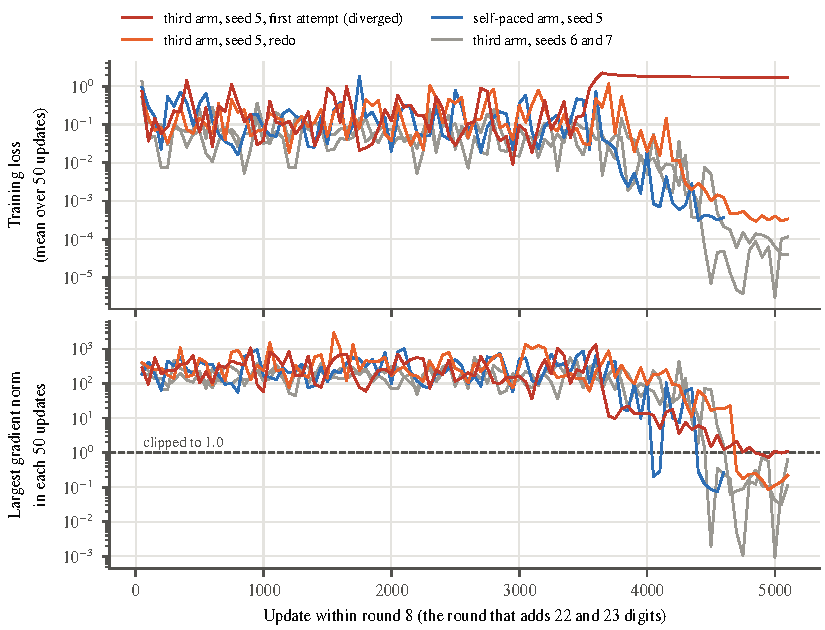
\includegraphics[width=\linewidth]{generated/figure_ladder_loss.pdf}
\caption{Training loss (top) and largest gradient norm before clipping
  (bottom) during round~8 of the ladder, per 50 updates.}
\label{fig:ladder-loss}
\end{figure}
